%%%%%%%%%%%%%%%%%%%%%%%%%%%%%%%%%%%%%%%%%
% Beamer Presentation
% LaTeX Template
% Version 1.0 (10/11/12)
%
% This template has been downloaded from:
% http://www.LaTeXTemplates.com
%
% License:
% CC BY-NC-SA 3.0 (http://creativecommons.org/licenses/by-nc-sa/3.0/)
%
%%%%%%%%%%%%%%%%%%%%%%%%%%%%%%%%%%%%%%%%%

%----------------------------------------------------------------------------------------
%	PACKAGES AND THEMES
%----------------------------------------------------------------------------------------

\documentclass[UTF8,aspectratio=169,14pt]{ctexbeamer}

\usepackage{hyperref}
\hypersetup{
	colorlinks=true,
	linkcolor=red,
	anchorcolor=blue,
	citecolor=green
}

\mode<presentation> {
	
	% The Beamer class comes with a number of default slide themes
	% which change the colors and layouts of slides. Below this is a list
	% of all the themes, uncomment each in turn to see what they look like.
	
	%\usetheme{default}
	%\usetheme{AnnArbor}
	%\usetheme{Antibes}
	%\usetheme{Bergen}
	%\usetheme{Berkeley}
	%\usetheme{Berlin}
	%\usetheme{Boadilla}
	%\usetheme{CambridgeUS}
	%\usetheme{Copenhagen}
	%\usetheme{Darmstadt}
	%\usetheme{Dresden}
	%\usetheme{Frankfurt}
	%\usetheme{Goettingen}
	%\usetheme{Hannover}
	%\usetheme{Ilmenau}
	%\usetheme{JuanLesPins}
	%\usetheme{Luebeck}
	\usetheme{Madrid}
	%\usetheme{Malmoe}
	%\usetheme{Marburg}
	%\usetheme{Montpellier}
	%\usetheme{PaloAlto}
	%\usetheme{Pittsburgh}
	%\usetheme{Rochester}
	%\usetheme{Singapore}
	%\usetheme{Szeged}
	%\usetheme{Warsaw}
	
	% As well as themes, the Beamer class has a number of color themes
	% for any slide theme. Uncomment each of these in turn to see how it
	% changes the colors of your current slide theme.
	
	%\usecolortheme{albatross}
	%\usecolortheme{beaver}
	%\usecolortheme{beetle}
	%\usecolortheme{crane}
	%\usecolortheme{dolphin}
	%\usecolortheme{dove}
	%\usecolortheme{fly}
	%\usecolortheme{lily}
	%\usecolortheme{orchid}
	%\usecolortheme{rose}
	%\usecolortheme{seagull}
	%\usecolortheme{seahorse}
	%\usecolortheme{whale}
	%\usecolortheme{wolverine}
	
	%\setbeamertemplate{footline} % To remove the footer line in all slides uncomment this line
	%\setbeamertemplate{footline}[page number] % To replace the footer line in all slides with a simple slide count uncomment this line
	
	%\setbeamertemplate{navigation symbols}{} % To remove the navigation symbols from the bottom of all slides uncomment this line
}

\usepackage{graphicx} % Allows including images
\graphicspath{{./figs/}}
\usepackage{booktabs} % Allows the use of \toprule, \midrule and \bottomrule in tables
\usepackage{longtable}
\usepackage{listings}
\usepackage{xcolor}
\lstset{numbers=left, %设置行号位置
	numberstyle=\tiny, %设置行号大小
	keywordstyle=\color{blue}, %设置关键字颜色
	commentstyle=\color[cmyk]{1,0,1,0}, %设置注释颜色
	frame=single, %设置边框格式
	escapeinside=``, %逃逸字符(1左面的键),用于显示中文
	%breaklines, %自动折行
	extendedchars=false, %解决代码跨页时,章节标题,页眉等汉字不显示的问题
	xleftmargin=2em,xrightmargin=2em, aboveskip=1em, %设置边距
	tabsize=4, %设置tab空格数
	showspaces=false %不显示空格
}
% Fonts
% \usepackage{libertine}
% \setmonofont{Courier}
\setCJKsansfont[ItalicFont=Noto Serif CJK SC Black, BoldFont=Noto Sans CJK SC Black]{Noto Sans CJK SC}


%----------------------------------------------------------------------------------------
%	TITLE PAGE
%----------------------------------------------------------------------------------------

\title[第14讲]{第十四讲 :信号量与管程} % The short title appears at the bottom of every slide, the full title is only on the title page
\subtitle{第6节:Rust语言中的同步机制}
\author{向勇、陈渝、李国良} % Your name
\institute[清华大学] % Your institution as it will appear on the bottom of every slide, may be shorthand to save space
{
	清华大学计算机系 \\ % Your institution for the title page
	\medskip
	\textit{xyong,yuchen,liguoliang@tsinghua.edu.cn} % Your email address
}
\date{\today} % Date, can be changed to a custom date


\begin{document}

\begin{frame}
\titlepage % Print the title page as the first slide
\end{frame}

%----------------------------------------------
\begin{frame}
\frametitle{提纲} % Table of contents slide, comment this block out to remove it
\tableofcontents % Throughout your presentation, if you choose to use \section{} and \subsection{} commands, these will automatically be printed on this slide as an overview of your presentation
\end{frame}
%----------------------------------------------
%%	PRESENTATION SLIDES
%----------------------------------------------
\section{第6节:Rust语言中的同步机制} % Sections can be created in order to organize your presentation into discrete blocks, all sections and subsections are automatically printed in the table of contents as an overview of the talk
%----------------------------------------------
\subsection{引用计数} % A subsection can be created just before a set of slides with a common theme to further break down your presentation into chunks
%----------------------------------------------
\begin{frame}[fragile]
    \frametitle{\href{https://doc.rust-lang.org/std/sync/index.html}{Higher-level synchronization objects in Rust}}
%    \framesubtitle{xxxx}

%% itemize
    \begin{itemize}
        \item Arc: A thread-safe atomically Reference-Counted pointer, which can be used in multithreaded environments. \pause
        \item Barrier: Ensures multiple threads will wait for each other to reach a point in the program, before continuing execution all together. \pause
        \item Condvar: Condition Variable, providing the ability to block a thread while waiting for an event to occur. \pause
        \item Mutex: Mutual Exclusion mechanism, which ensures that at most one thread at a time is able to access some data. \pause
        \item RwLock: Provides a mutual exclusion mechanism which allows multiple readers at the same time, while allowing only one writer at a time.
    \end{itemize}

%% figure
%    \begin{figure}
%    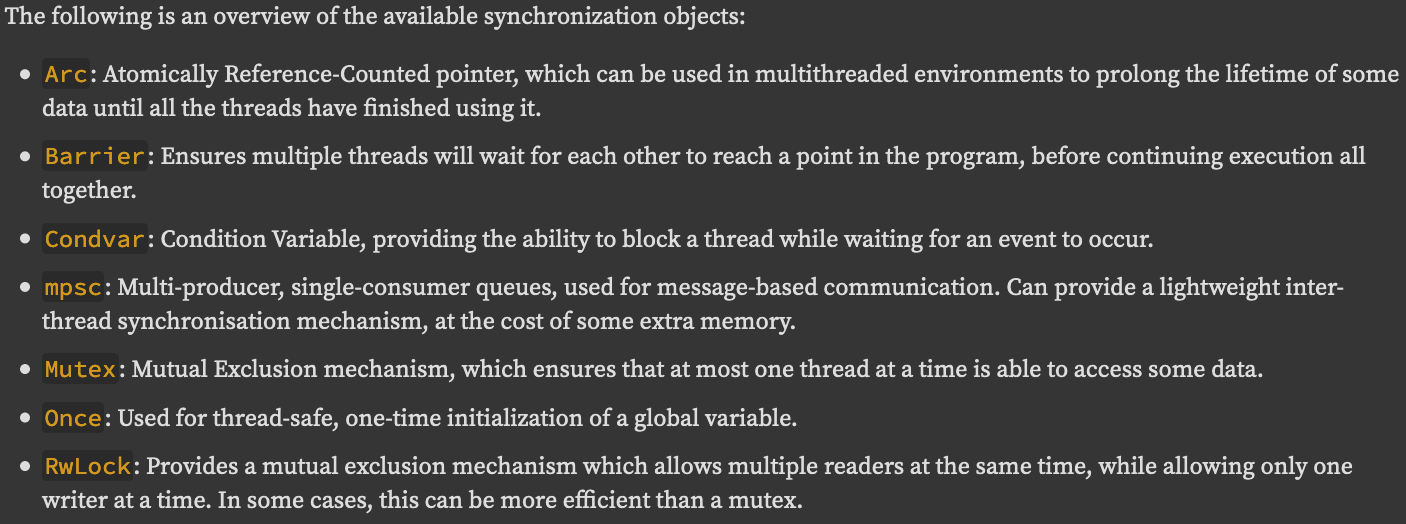
\includegraphics[width=1.0\linewidth]{figs/sync-obj.png}
%    \caption{xxxx}
%    \end{figure}

\end{frame}
%----------------------------------------------
% ## 第十四讲 信号量与管程
% 
% ### 14.6 Synchronization in Rust
% 
% #### Higher-level synchronization objects in Rust
% 
% https://doc.rust-lang.org/std/sync/index.html#higher-level-synchronization-objects
% Higher-level synchronization objects
% 
% ![sync-obj](figs/sync-obj.png)
% 
% Arc: A thread-safe reference-counting pointer.
% 
% Atomically Reference-Counted pointer, which can be used in multithreaded environments to prolong the lifetime of some data until all the threads have finished using it.
% 
% Barrier: Ensures multiple threads will wait for each other to reach a point in the program, before continuing execution all together.
% 
% Condvar: Condition Variable, providing the ability to block a thread while waiting for an event to occur.
% 
% mpsc: Multi-producer, single-consumer queues, used for message-based communication. Can provide a lightweight inter-thread synchronisation mechanism, at the cost of some extra memory.
% 
% Mutex: Mutual Exclusion mechanism, which ensures that at most one thread at a time is able to access some data.
% 
% Once: Used for thread-safe, one-time initialization of a global variable.
% 
% RwLock: Provides a mutual exclusion mechanism which allows multiple readers at the same time, while allowing only one writer at a time. In some cases, this can be more efficient than a mutex.
% 
%----------------------------------------------
\begin{frame}[fragile]
    \frametitle{\href{https://doc.rust-lang.org/rust-by-example/std/rc.html}{Rc(Reference Counting)}}
%    \framesubtitle{yyyy}

A single-threaded reference-counting pointer. 'Rc' stands for 'Reference Counted'.

 \pause
 
%% figure
    \begin{figure}
    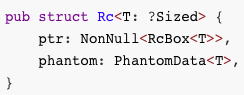
\includegraphics[width=0.4\linewidth]{figs/struct-rc.png}
%    \caption{xxxx}
    \end{figure}

\end{frame}
%----------------------------------------------
% #### Rc:单线程引用计数
% 
% https://doc.rust-lang.org/rust-by-example/std/rc.html
% Rc(Reference Counting)
% 
% A single-threaded reference-counting pointer. 'Rc' stands for 'Reference Counted'.
% 
% https://doc.rust-lang.org/1.37.0/src/alloc/rc.rs.html#273-276
% 
% ![struct-rc](figs/struct-rc.png)
% 
% ```rust
% pub struct Rc<T: ?Sized> {
%     ptr: NonNull<RcBox<T>>,
%     phantom: PhantomData<T>,
% }
% ```
% 
%----------------------------------------------
\begin{frame}[fragile]
    \frametitle{\href{https://doc.rust-lang.org/rust-by-example/std/rc.html}{Example of Reference Counting}}
%    \framesubtitle{yyyy}
%% figure
    \begin{figure}
    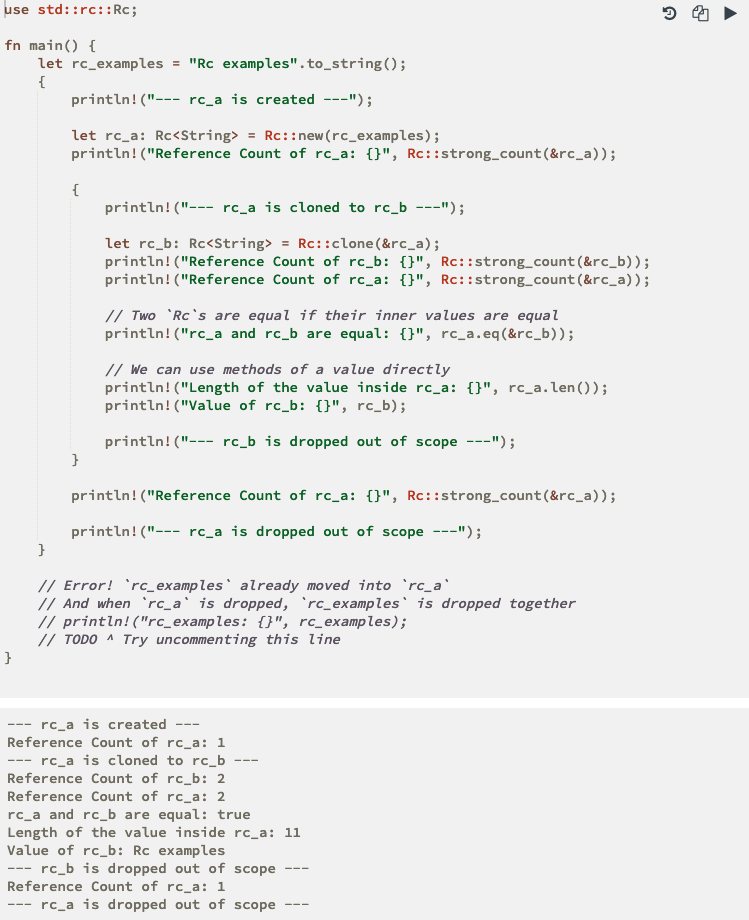
\includegraphics[width=0.37\linewidth]{figs/rc-example.png}
%    \caption{xxxx}
    \end{figure}

\end{frame}
%----------------------------------------------
% #### Example of Reference Counting
% 
% ![rc-example](figs/rc-example.png)
% 
% 
% 
%----------------------------------------------
\begin{frame}[fragile]
    \frametitle{\href{https://doc.rust-lang.org/std/sync/struct.Arc.html}{Arc: Atomically Reference-Counted pointer}}
%    \framesubtitle{yyyy}

A thread-safe reference-counting pointer. 'Arc' stands for 'Atomically Reference Counted'. \pause

%% figure
    \begin{figure}
    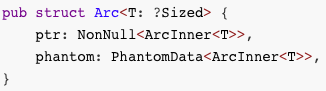
\includegraphics[width=0.5\linewidth]{figs/struct-arc.png}
%    \caption{xxxx}
    \end{figure}

\end{frame}
%----------------------------------------------
% #### Arc: Atomically Reference-Counted pointer
% 
% https://doc.rust-lang.org/std/sync/struct.Arc.html
% Struct std::sync::Arc
% 
% A thread-safe reference-counting pointer. 'Arc' stands for 'Atomically Reference Counted'.
% 
% https://doc.rust-lang.org/src/alloc/sync.rs.html#196-199
% 
% ![struct-arc](figs/struct-arc.png)
% 
% ```rust
% pub struct Arc<T: ?Sized> {
%     ptr: NonNull<ArcInner<T>>,
%     phantom: PhantomData<ArcInner<T>>,
% }
% ```
% 
%----------------------------------------------
\begin{frame}[fragile]
    \frametitle{Methods in std::sync::Arc}
%    \framesubtitle{yyyy}
%% figure
    \begin{figure}
    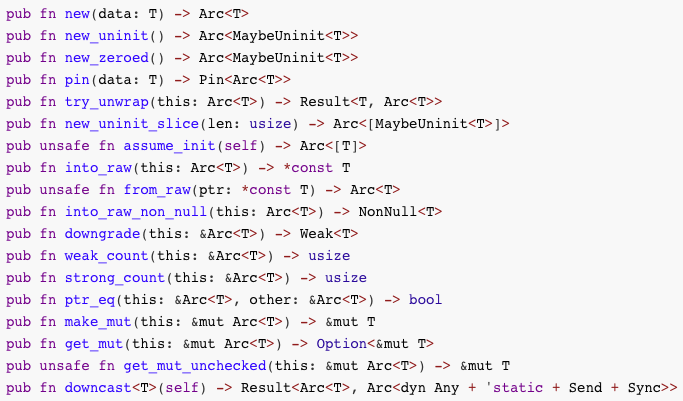
\includegraphics[width=0.8\linewidth]{figs/methods-arc.png}
%    \caption{xxxx}
    \end{figure}

\end{frame}
%----------------------------------------------
% ![methods-arc](figs/methods-arc.png)
% 
% ```rust
% pub fn new(data: T) -> Arc<T>
% pub fn new_uninit() -> Arc<MaybeUninit<T>>
% pub fn new_zeroed() -> Arc<MaybeUninit<T>>
% pub fn pin(data: T) -> Pin<Arc<T>>
% pub fn try_unwrap(this: Arc<T>) -> Result<T, Arc<T>>
% pub fn new_uninit_slice(len: usize) -> Arc<[MaybeUninit<T>]>
% pub unsafe fn assume_init(self) -> Arc<[T]>
% pub fn into_raw(this: Arc<T>) -> *const T
% pub unsafe fn from_raw(ptr: *const T) -> Arc<T>
% pub fn into_raw_non_null(this: Arc<T>) -> NonNull<T>
% pub fn downgrade(this: &Arc<T>) -> Weak<T>
% pub fn weak_count(this: &Arc<T>) -> usize
% pub fn strong_count(this: &Arc<T>) -> usize
% pub fn ptr_eq(this: &Arc<T>, other: &Arc<T>) -> bool
% pub fn make_mut(this: &mut Arc<T>) -> &mut T
% pub fn get_mut(this: &mut Arc<T>) -> Option<&mut T>
% pub unsafe fn get_mut_unchecked(this: &mut Arc<T>) -> &mut T
% pub fn downcast<T>(self) -> Result<Arc<T>, Arc<dyn Any + 'static + Send + Sync>> 
% ```
% 
% https://doc.rust-lang.org/src/alloc/sync.rs.html#943
% fn clone(&self)
% 
%----------------------------------------------
\subsection{原子操作} % A subsection can be created just before a set of slides with a common theme to further break down your presentation into chunks
%----------------------------------------------
\begin{frame}
\frametitle{提纲} % Table of contents slide, comment this block out to remove it
\tableofcontents % Throughout your presentation, if you choose to use \section{} and \subsection{} commands, these will automatically be printed on this slide as an overview of your presentation
\end{frame}
%----------------------------------------------
\begin{frame}[fragile]
    \frametitle{\href{https://doc.rust-lang.org/core/sync/atomic/index.html}{Atomic}}
%    \framesubtitle{yyyy}

Atomic types provide primitive shared-memory communication between threads, and are the building blocks of other concurrent types.

%% figure
    \begin{figure}
    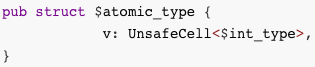
\includegraphics[width=0.5\linewidth]{figs/struct-atomic.png}
%    \caption{xxxx}
    \end{figure}

\end{frame}
%----------------------------------------------
% #### atomic(原子操作)
% https://doc.rust-lang.org/core/sync/atomic/index.html
% Module core::sync::atomic
% 
% Atomic types provide primitive shared-memory communication between threads, and are the building blocks of other concurrent types.
% 
% https://doc.rust-lang.org/src/core/sync/atomic.rs.html#1229-1231
% 
% ![struct-atomic](figs/struct-atomic.png)
% 
% ```rust
% pub struct $atomic_type {
%             v: UnsafeCell<$int_type>,
% }
% ```
% 
%----------------------------------------------
\begin{frame}[fragile]
    \frametitle{Methods in Atomic}
%    \framesubtitle{yyyy}
%% figure
    \begin{figure}
    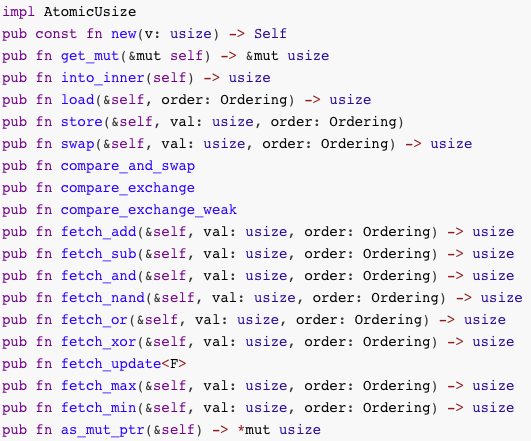
\includegraphics[width=0.55\linewidth]{figs/methods-atomic.png}
%    \caption{xxxx}
    \end{figure}

\end{frame}
%----------------------------------------------
% ![methods-atomic](figs/methods-atomic.png)
% 
% 
% ```rust
% impl AtomicUsize
% pub const fn new(v: usize) -> Self
% pub fn get_mut(&mut self) -> &mut usize
% pub fn into_inner(self) -> usize
% pub fn load(&self, order: Ordering) -> usize
% pub fn store(&self, val: usize, order: Ordering)
% pub fn swap(&self, val: usize, order: Ordering) -> usize
% pub fn compare_and_swap
% pub fn compare_exchange
% pub fn compare_exchange_weak
% pub fn fetch_add(&self, val: usize, order: Ordering) -> usize
% pub fn fetch_sub(&self, val: usize, order: Ordering) -> usize
% pub fn fetch_and(&self, val: usize, order: Ordering) -> usize
% pub fn fetch_nand(&self, val: usize, order: Ordering) -> usize
% pub fn fetch_or(&self, val: usize, order: Ordering) -> usize
% pub fn fetch_xor(&self, val: usize, order: Ordering) -> usize
% pub fn fetch_update<F>
% pub fn fetch_max(&self, val: usize, order: Ordering) -> usize
% pub fn fetch_min(&self, val: usize, order: Ordering) -> usize
% pub fn as_mut_ptr(&self) -> *mut usize
% ```
% 
%----------------------------------------------
\subsection{执行同步} % A subsection can be created just before a set of slides with a common theme to further break down your presentation into chunks
%----------------------------------------------
\begin{frame}
\frametitle{提纲} % Table of contents slide, comment this block out to remove it
\tableofcontents % Throughout your presentation, if you choose to use \section{} and \subsection{} commands, these will automatically be printed on this slide as an overview of your presentation
\end{frame}
%----------------------------------------------
\begin{frame}[fragile]
    \frametitle{\href{https://doc.rust-lang.org/std/sync/struct.Barrier.html}{Barrier}}
%    \framesubtitle{yyyy}

A barrier enables multiple threads to synchronize the beginning of some computation. \pause

%% figure
    \begin{figure}
    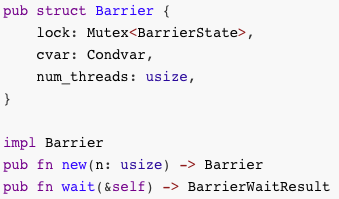
\includegraphics[width=0.6\linewidth]{figs/struct-barrier.png}
%    \caption{xxxx}
    \end{figure}

\end{frame}
%----------------------------------------------
% #### Barrier(内存屏障)
% 
% https://doc.rust-lang.org/std/sync/struct.Barrier.html
% Struct std::sync::Barrier
% 
% A barrier enables multiple threads to synchronize the beginning of some computation.
% 
% ![struct-barrier](figs/struct-barrier.png)
% 
% ```rust
% pub struct Barrier {
%     lock: Mutex<BarrierState>,
%     cvar: Condvar,
%     num_threads: usize,
% }
% 
% impl Barrier
% pub fn new(n: usize) -> Barrier
% pub fn wait(&self) -> BarrierWaitResult
% ```
% 
%----------------------------------------------
\begin{frame}[fragile]
    \frametitle{\href{https://doc.rust-lang.org/std/sync/struct.Barrier.html}{Example of Barrier}}
%    \framesubtitle{yyyy}
%% figure
    \begin{figure}
    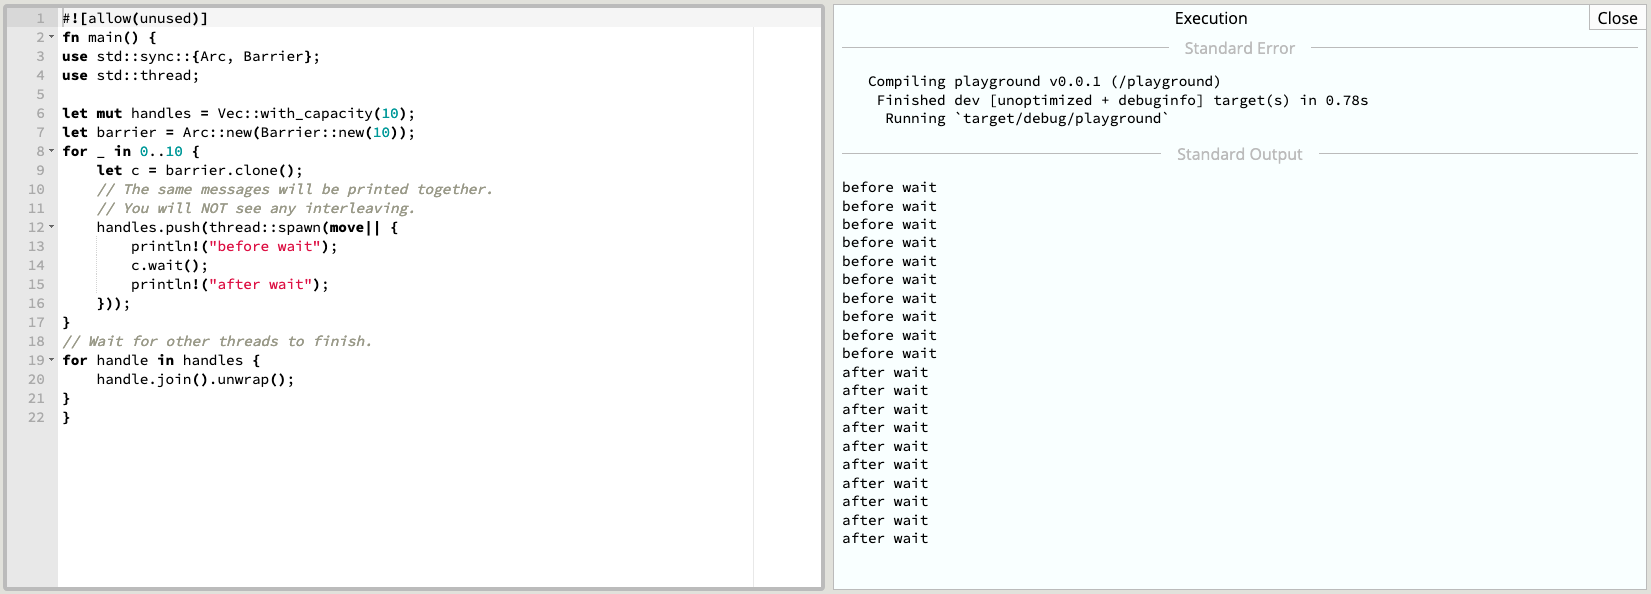
\includegraphics[width=1.0\linewidth]{figs/demo-barrier.png}
%    \caption{xxxx}
    \end{figure}

\end{frame}
%----------------------------------------------
% ##### Example of Barrier
% 
% https://doc.rust-lang.org/std/sync/struct.Barrier.html
% 
% 有一个例子可演示;
% 
% ![demo-barrier](figs/demo-barrier.png)
% 
% https://doc.rust-lang.org/src/std/sync/barrier.rs.html#128-145
% pub fn wait(&self) -> BarrierWaitResult
% 
% lock = self.cvar.wait(lock).unwrap();
% 
%----------------------------------------------
\subsection{条件变量} % A subsection can be created just before a set of slides with a common theme to further break down your presentation into chunks
%----------------------------------------------
\begin{frame}
\frametitle{提纲} % Table of contents slide, comment this block out to remove it
\tableofcontents % Throughout your presentation, if you choose to use \section{} and \subsection{} commands, these will automatically be printed on this slide as an overview of your presentation
\end{frame}
%----------------------------------------------
\begin{frame}[fragile]
    \frametitle{\href{https://doc.rust-lang.org/std/sync/struct.Condvar.html}{Condvar}}
%    \framesubtitle{yyyy}

Condition variables represent the ability to block a thread such that it consumes no CPU time while waiting for an event to occur. \pause

%% figure
    \begin{figure}
    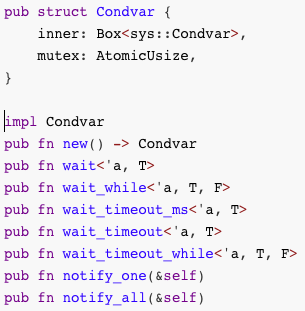
\includegraphics[width=0.37\linewidth]{figs/struct-condvar.png}
%    \caption{xxxx}
    \end{figure}

\end{frame}
%----------------------------------------------
% #### Condvar(条件变量)
% 
% https://doc.rust-lang.org/std/sync/struct.Condvar.html
% Struct std::sync::Condvar
% 
% Condition variables represent the ability to block a thread such that it consumes no CPU time while waiting for an event to occur. Condition variables are typically associated with a boolean predicate (a condition) and a mutex. The predicate is always verified inside of the mutex before determining that a thread must block.
% 
% ![struct-condvar](figs/struct-condvar.png)
% 
% ```rust
% pub struct Condvar {
%     inner: Box<sys::Condvar>,
%     mutex: AtomicUsize,
% }
% 
% impl Condvar
% pub fn new() -> Condvar
% pub fn wait<'a, T>
% pub fn wait_while<'a, T, F>
% pub fn wait_timeout_ms<'a, T>
% pub fn wait_timeout<'a, T>
% pub fn wait_timeout_while<'a, T, F>
% pub fn notify_one(&self)
% pub fn notify_all(&self)
% ```
% 
% ```rust 
% 
% ```
%----------------------------------------------
\begin{frame}[fragile]
    \frametitle{Example of Condvar}
%    \framesubtitle{yyyy}
%% figure
    \begin{figure}
    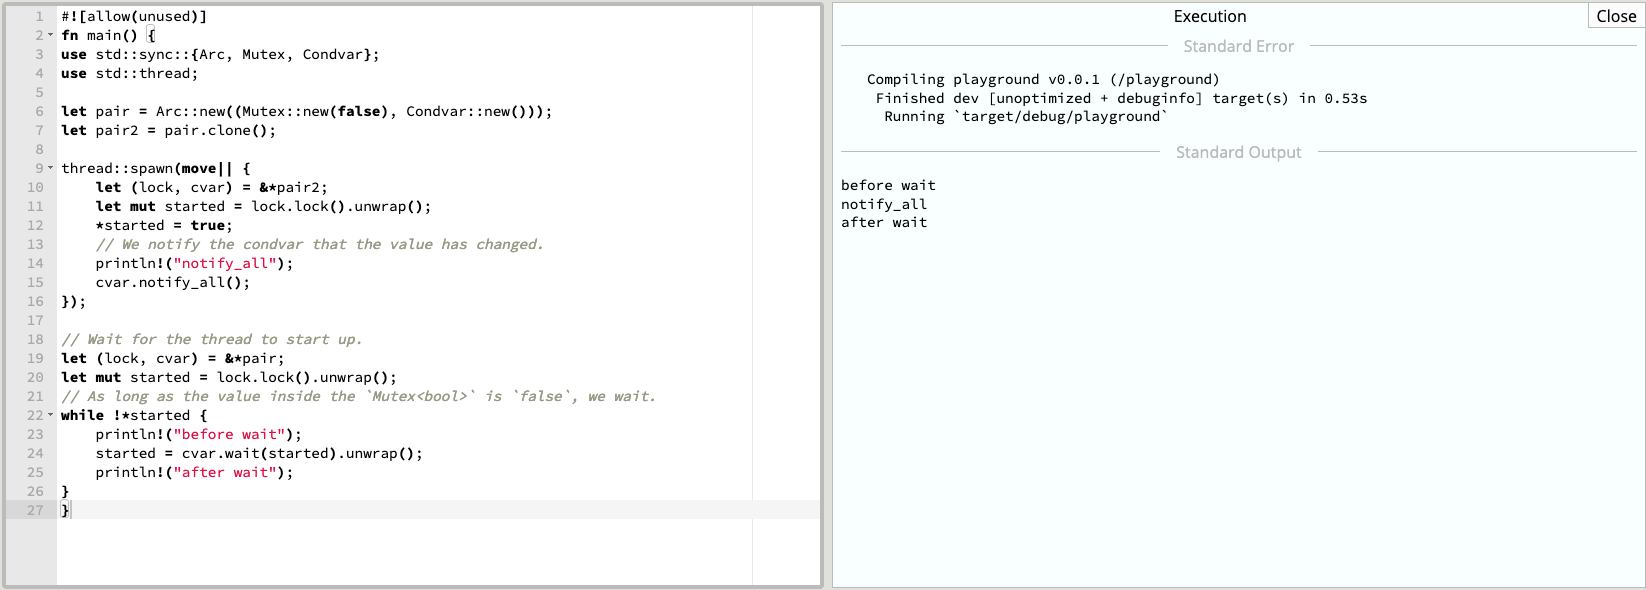
\includegraphics[width=1.0\linewidth]{figs/demo-condvar.png}
%    \caption{xxxx}
    \end{figure}

\end{frame}
%----------------------------------------------
% ##### Example of Condvar
% 
% ![demo-condvar](figs/demo-condvar.png)
% 
% ```rust
% #![allow(unused)]
% fn main() {
% use std::sync::{Arc, Mutex, Condvar};
% use std::thread;
% 
% let pair = Arc::new((Mutex::new(false), Condvar::new()));
% let pair2 = pair.clone();
% 
% thread::spawn(move|| {
%     let (lock, cvar) = &*pair2;
%     let mut started = lock.lock().unwrap();
%     *started = true;
%     // We notify the condvar that the value has changed.
%     println!("notify_all");
%     cvar.notify_all();
% });
% 
% // Wait for the thread to start up.
% let (lock, cvar) = &*pair;
% let mut started = lock.lock().unwrap();
% // As long as the value inside the `Mutex<bool>` is `false`, we wait.
% while !*started {
%     println!("before wait");
%     started = cvar.wait(started).unwrap();
%     println!("after wait");
% }
% }
% ```
%----------------------------------------------
\subsection{互斥信号量} % A subsection can be created just before a set of slides with a common theme to further break down your presentation into chunks
%----------------------------------------------
\begin{frame}
\frametitle{提纲} % Table of contents slide, comment this block out to remove it
\tableofcontents % Throughout your presentation, if you choose to use \section{} and \subsection{} commands, these will automatically be printed on this slide as an overview of your presentation
\end{frame}
%----------------------------------------------
\begin{frame}[fragile]
    \frametitle{\href{https://doc.rust-lang.org/std/sync/struct.Mutex.html}{Mutex}}
%    \framesubtitle{yyyy}

A mutual exclusion primitive useful for protecting shared data. \pause

\begin{columns}[c] % The "c" option specifies centered vertical alignment while the "t" option is used for top vertical alignment

\column{.4\textwidth} % Left column and width

%% figure
    \begin{figure}
    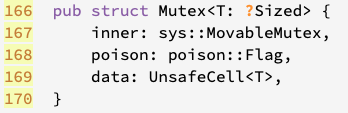
\includegraphics[width=0.9\linewidth]{figs/mutex-struct.png}
%    \caption{xxxx}
    \end{figure}

\column{.6\textwidth} % Right column and width

%% figure
    \begin{figure}
    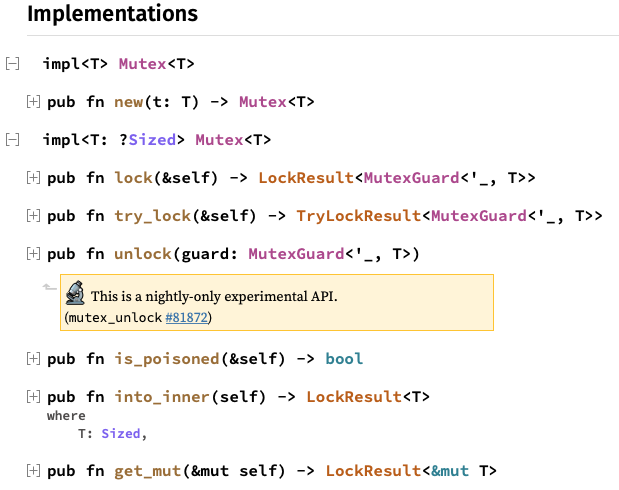
\includegraphics[width=0.9\linewidth]{figs/mutex-implement.png}
%    \caption{xxxx}
    \end{figure}

\end{columns}

\end{frame}
%----------------------------------------------
% #### Mutex(互斥信号量)
% 
% https://doc.rust-lang.org/std/sync/struct.Mutex.html
% Struct std::sync::Mutex
% A mutual exclusion primitive useful for protecting shared data
% 
% 这里有mutex的例子和实现描述;
% 
% https://doc.rust-lang.org/src/std/sync/mutex.rs.html#111
% struct Mutex的实现
% 
% 
% 
% ![struct-mutex](figs/struct-mutex.png)
% 
% ```rust
% pub struct Mutex<T: ?Sized> {
%     // Note that this mutex is in a *box*, not inlined into the struct itself.
%     // Once a native mutex has been used once, its address can never change (it
%     // can't be moved). This mutex type can be safely moved at any time, so to
%     // ensure that the native mutex is used correctly we box the inner mutex to
%     // give it a constant address.
%     inner: Box<sys::Mutex>,
%     poison: poison::Flag,
%     data: UnsafeCell<T>,
% }
% 
% impl<T> Mutex<T>
% pub fn new(t: T) -> Mutex<T>
% pub fn lock(&self) -> LockResult<MutexGuard<T>>
% pub fn try_lock(&self) -> TryLockResult<MutexGuard<T>>
% pub fn is_poisoned(&self) -> bool
% pub fn into_inner(self) -> LockResult<T>
% pub fn get_mut(&mut self) -> LockResult<&mut T>
% ```
% 
%----------------------------------------------
\subsection{读写锁} % A subsection can be created just before a set of slides with a common theme to further break down your presentation into chunks
%----------------------------------------------
\begin{frame}[fragile]
    \frametitle{\href{https://doc.rust-lang.org/std/sync/struct.RwLock.html}{RwLock}}
%    \framesubtitle{yyyy}

Rwlock allows a number of readers or at most one writer at any point in time. The write portion of this lock typically allows modification of the underlying data (exclusive access). \pause

%% figure
    \begin{figure}
    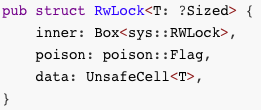
\includegraphics[width=0.5\linewidth]{figs/struct-rwlock.png}
%    \caption{xxxx}
    \end{figure}

\end{frame}
%----------------------------------------------
% #### RwLock(读写锁)
% 
% https://doc.rust-lang.org/std/sync/struct.RwLock.html
% Struct std::sync::RwLock
% 
% This type of lock allows a number of readers or at most one writer at any point in time. The write portion of this lock typically allows modification of the underlying data (exclusive access) and the read portion of this lock typically allows for read-only access (shared access).
% 
% ![struct-rwlock](figs/struct-rwlock.png)
% 
% ```rust
% pub struct RwLock<T: ?Sized> {
%     inner: Box<sys::RWLock>,
%     poison: poison::Flag,
%     data: UnsafeCell<T>,
% }
% ```
%----------------------------------------------
\begin{frame}[fragile]
    \frametitle{Methods in Rwlock}
%    \framesubtitle{yyyy}
%% figure
    \begin{figure}
    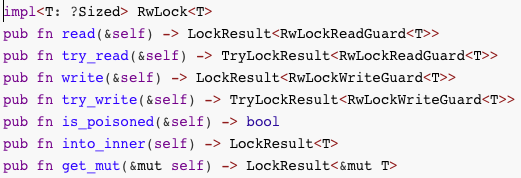
\includegraphics[width=1.0\linewidth]{figs/methods-rwlock.png}
%    \caption{xxxx}
    \end{figure}

\end{frame}
%----------------------------------------------
% ![methods-rwlock](figs/methods-rwlock.png)
% 
% ```rust
% impl<T: ?Sized> RwLock<T>
% pub fn read(&self) -> LockResult<RwLockReadGuard<T>>
% pub fn try_read(&self) -> TryLockResult<RwLockReadGuard<T>>
% pub fn write(&self) -> LockResult<RwLockWriteGuard<T>>
% pub fn try_write(&self) -> TryLockResult<RwLockWriteGuard<T>>
% pub fn is_poisoned(&self) -> bool
% pub fn into_inner(self) -> LockResult<T>
% pub fn get_mut(&mut self) -> LockResult<&mut T>
% ```
% 
%----------------------------------------------
\end{document}
